\begin{frame}{Oversigt over in-sample resultater}
%\begin{table}[ht] 
%\centering 
%\begin{tabular}{lll}
%\toprule 
%Inkluderingsrate & Variable & Beskrivelse \\ \midrule
%100\% &\textcolor{blue3}{CLF16OV} & Civilarbejdsstyrke \\
%100\% &\textcolor{blue3}{CE16OV} & Civilbeskæftigelse \\
%83.33\% & \textcolor{blue3}{lag 1} & Den tidligere værdi af arbejdsløshedsraten \\
%77.78\% & \textcolor{chartreuse4}{IPDMAT} & Holdbart materiale  \\
%77.78\% & \textcolor{blue3}{UEMPLT5} & Civile arbejdsløse - mindre end 5 uger \\
%77.78\% & \textcolor{blue3}{UEMP5TO14}& Civile arbejdsløse i 5 - 14 uger \\
%77.78\% & \textcolor{blue3}{UEMP15OV} &  Civile arbejdsløse i 15 - 26 uger  \\
%77.78\% & \textcolor{orange}{TB6MS} & 6-måneders statsskat  \\
%77.78\% & \textcolor{orange}{GS5} & 5-årig statsobligationsrente \\
%\bottomrule
%\end{tabular}  
%\caption{Inkluderingsraten af de 9 hyppigst valgte variable for de ialt 18 modeller samt beskrivelse af variablerne.}
%\end{table} 
\end{frame}

\begin{frame}{Oversigt over in-sample resultater}
\begin{figure}
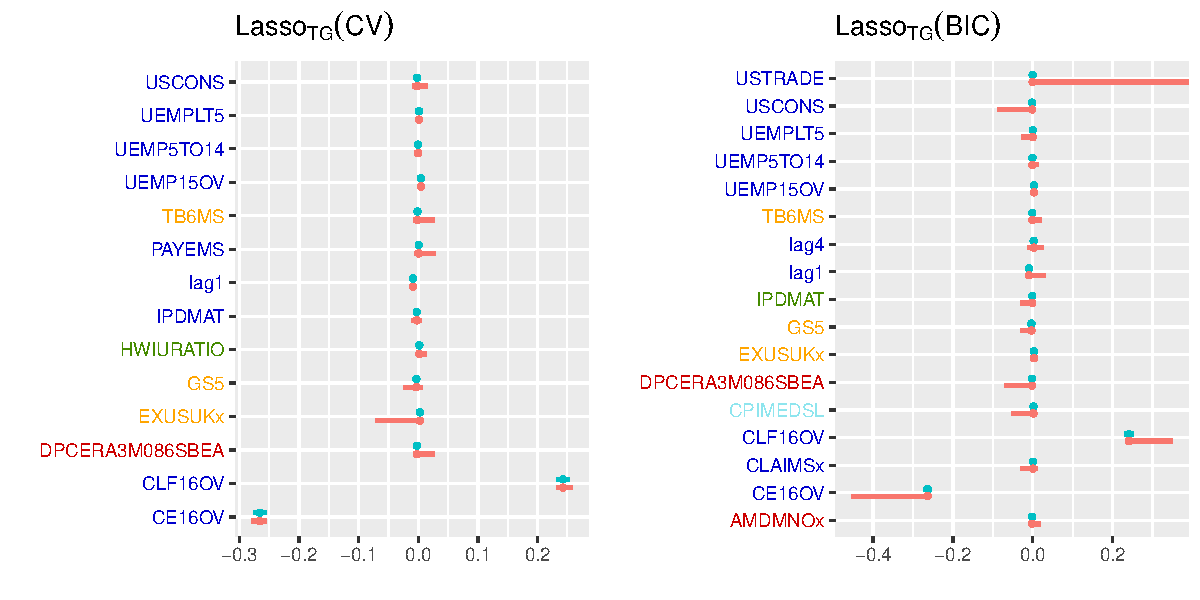
\includegraphics[width=1\linewidth, height=0.7\textheight]{slides/cf_interval.pdf}
\caption{Betinget 95\% konfidensinterval for lasso\(_{TG}\) (CV) og lasso\(_{TG}\) (BIC) (rød) og 95\% konfidensinterval for OLS estimatorerne for de udvalgte prædiktorer (blå).}
\end{figure}
\end{frame}


%%% Local Variables:
%%% mode: latex
%%% TeX-master: "../beamer"
%%% End:
